\let\cleardoublepage=\clearpage

\chapter{Constraining the Rotation Profile in a Low-Luminosity Subgiant with a Surface Rotation Measurement}
\label{chap:subgiant_ast}

\section*{Preamble}

Asteroseismic inference of the core and surface rotation of low-luminosity subgiants reveals that the core-to-surface rotation rate ratio is much smaller than state-of-the-art models of rotating stellar evolution predict \citep{deheuvels_seismic_2014, cantiello_angular_2014, eggenberger_asteroseismology_2019}.
This result implies that there is missing physics in our treatment of angular momentum transport.
One way to determine the source of the missing angular momentum transport is to look for signatures of those mechanisms in the shape of the rotation profile.
However, due to the limited number and low precision of observed rotational splitting of low-luminosity subgiants, constraints to the rotation profile are usually limited to two-zone (core and surface rotation rate) inferences \citep{deheuvels_seismic_2014}.

We find, assuming a model-motivated step-function rotation profile, a consistent degeneracy between the surface rotation rate and radial position of a strong rotational gradient when performing asteroseismic inference using the observed rotational splittings of a low-luminosity subgiant.
We show that we can leverage this degeneracy to place stronger constraints on the position of the strong rotational gradient with independent measurements of the surface rotation rate assuming representative precision.
Furthermore, we apply this approach to the observed rotational splittings and surface rotation rate of low-luminosity subgiant KIC~12508433 and obtain stronger constraints to the internal rotation profile.
We find decreased support for rotation profiles with strong rotational gradients in the core and $r/R\ > \ 0.4$, which suggests the data disfavours angular momentum transport via internal gravity waves \citep[e.g.,][]{pincon_can_2017} or magnetorotational instabilities \citep[e.g.,][]{spada_angular_2016,menou_magnetorotational_2006}.
The method applied in this work can readily be adopted in other works to more tightly constrain the internal rotation profiles of post-main sequence stars without the requirement for more data.

This chapter was originally published as:
\begin{quote}
	\citet{tanner_ast}
\end{quote}
and is presented in the form that it was published \update{in accordance with Monash University's thesis by submission guidelines.}

\newpage

%add figures and captions for the figure and table lists. but hide them.

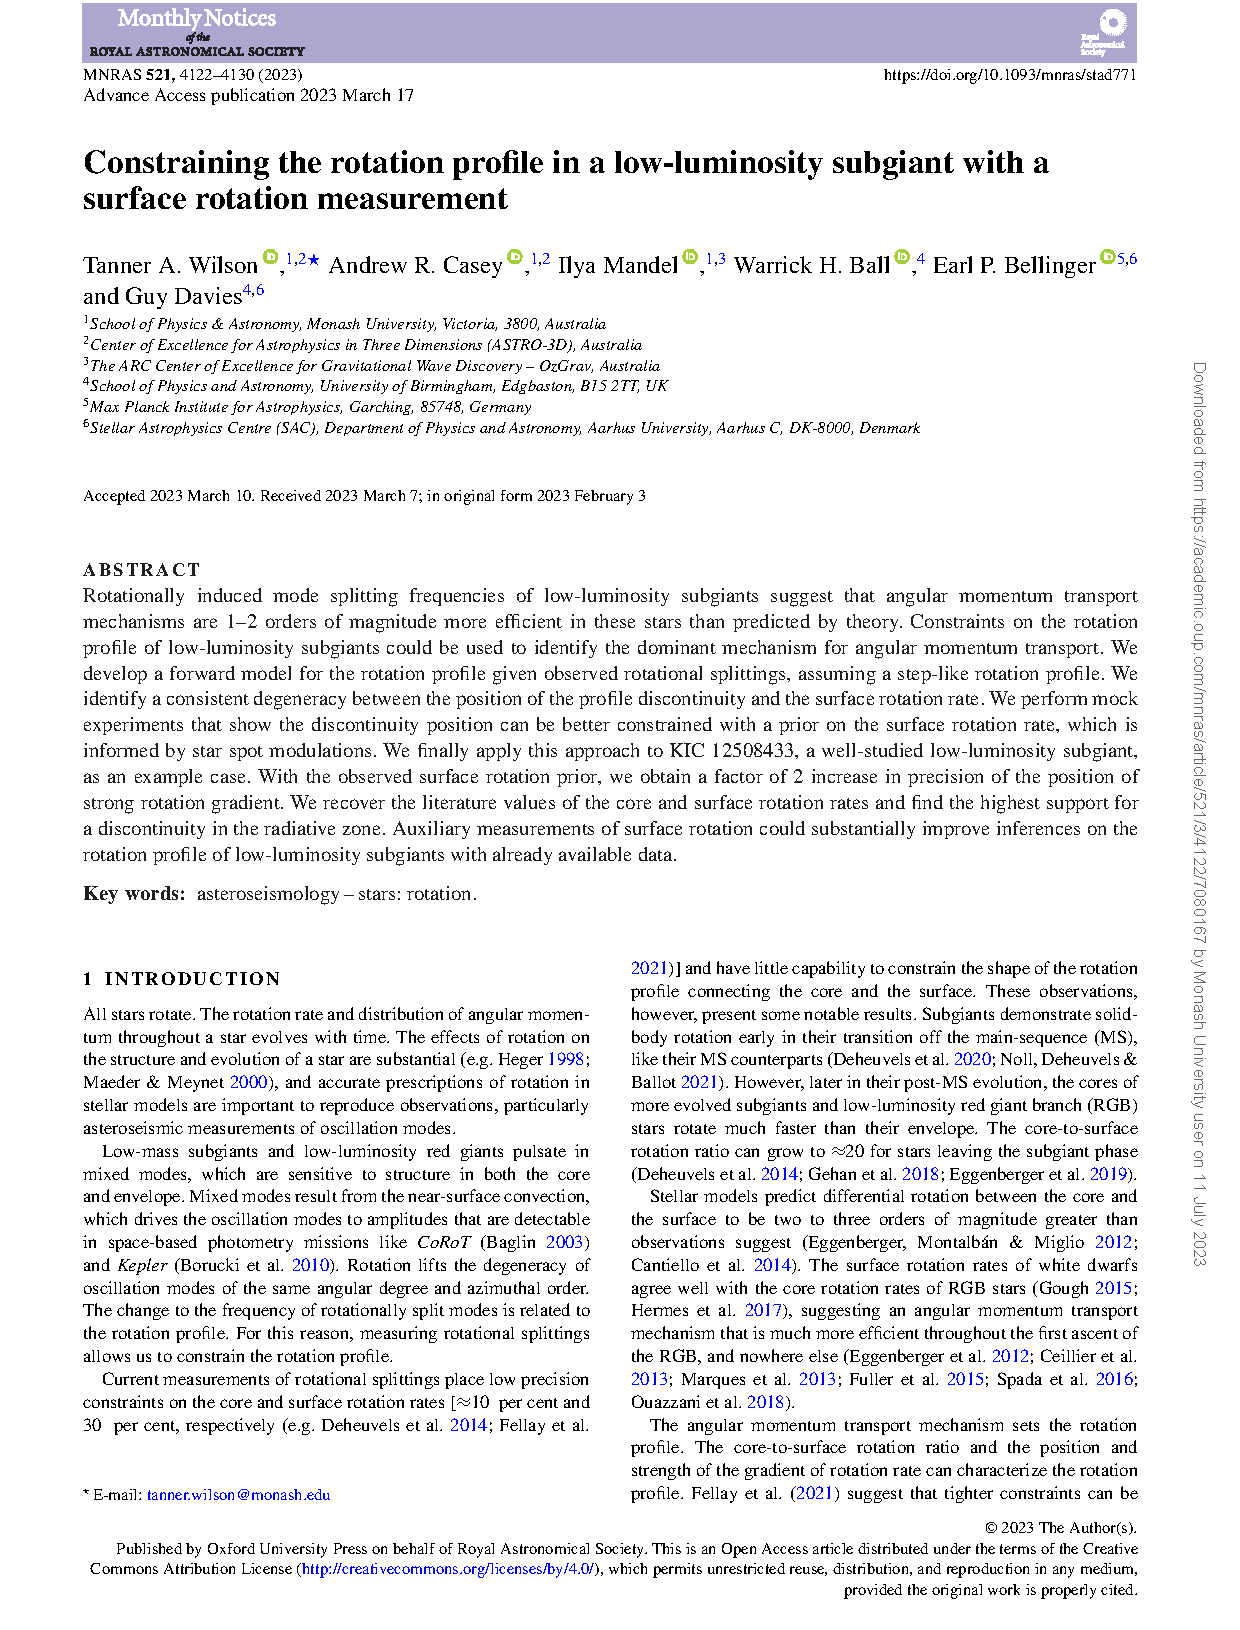
\includepdf[pages =1,addtotoc ={1,section,1, Introduction, p1}, scale=0.9,offset=65 -50,fitpaper=true]{Chapters/stad771-TW-subgiant.pdf}

\includepdf[pages =2,addtotoc ={2, subsection,2, Rotational Splittings, p1, 2, subsection,2, Forwards Model, p1 }, scale=0.9,offset=65 -50,fitpaper=true]{Chapters/stad771-TW-subgiant.pdf}

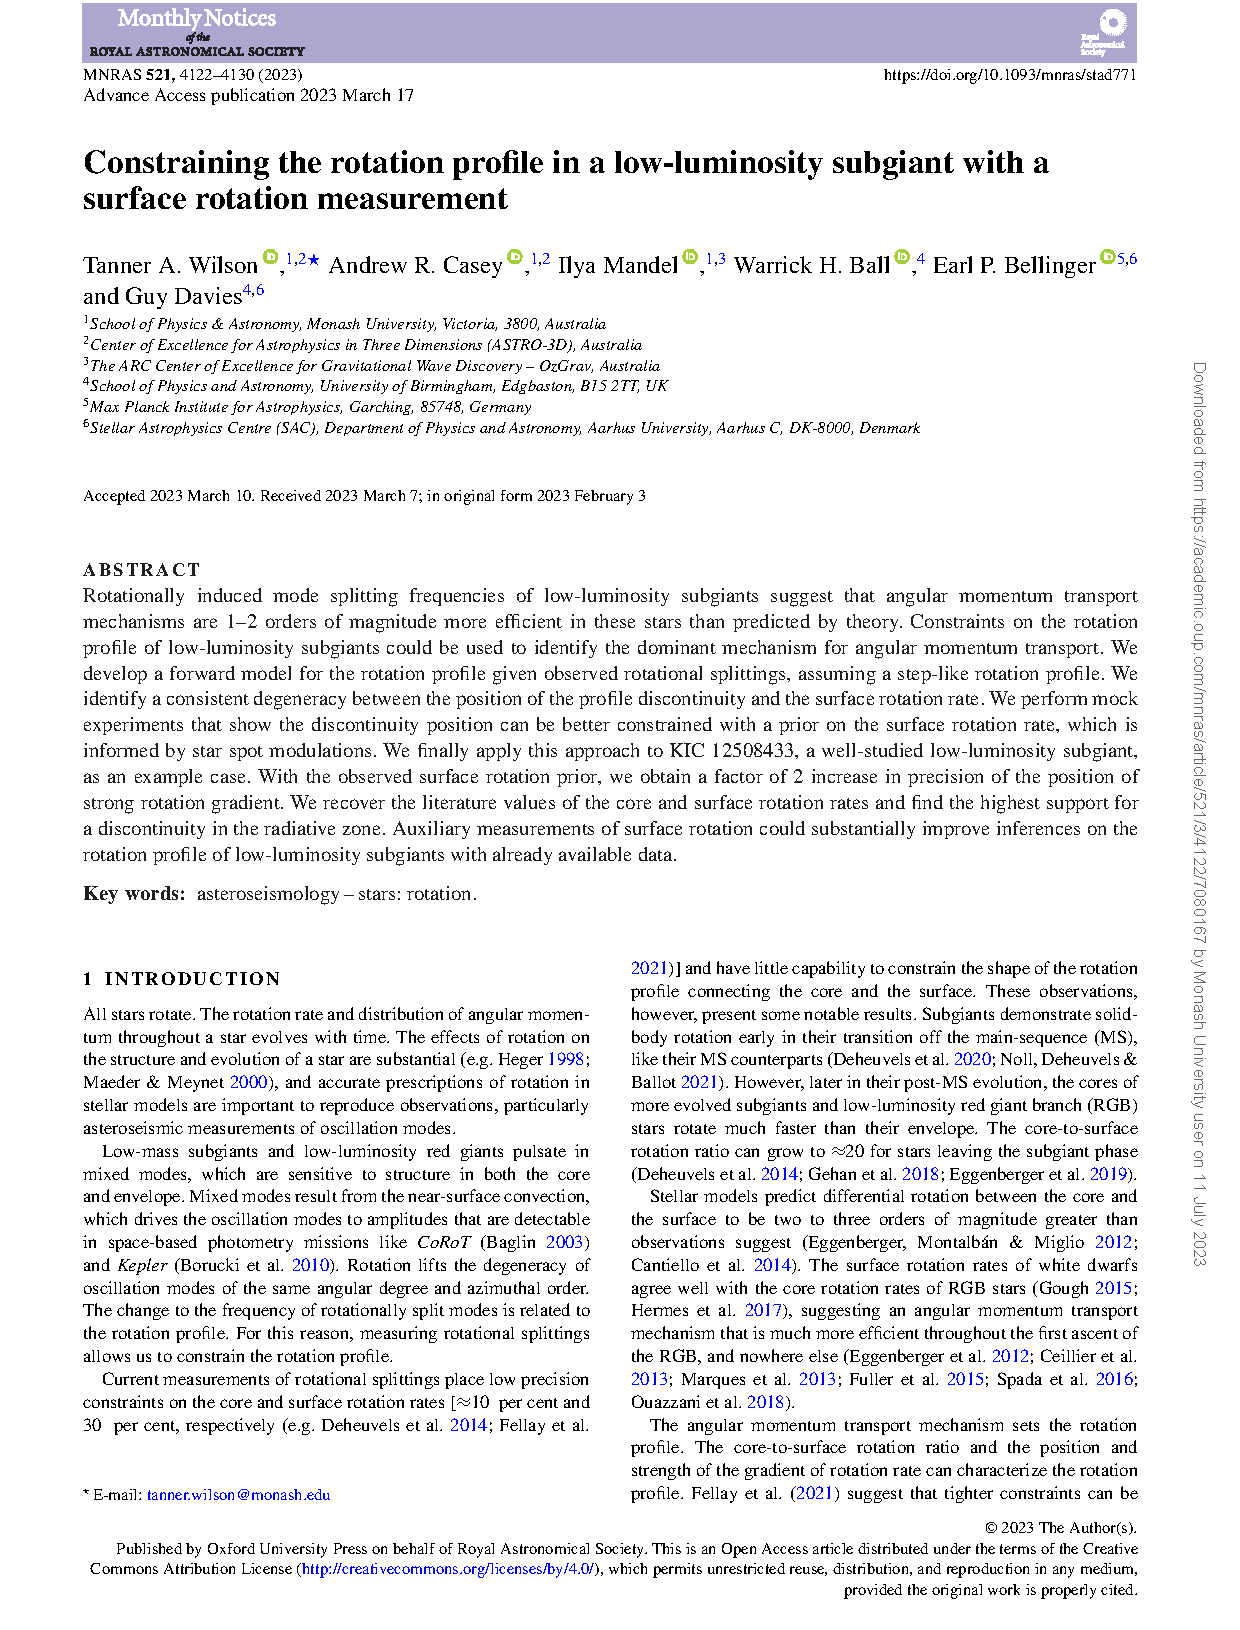
\includepdf[pages =3,addtotoc ={3, section, 1, Results, p1, 3, subsection,2, Mock data experiments with three hypothetical rotation profiles, p1 },addtolist={3, figure, Rotational kernels for the best-fitting model of KIC~12508433.,f1, 3,figure,Three rotation profiles used in the mock data experiments.,f1, 3,table,Measured properties and best-fit stellar model parameters of KIC~12508433.,t1}, scale=0.9,offset=65 -50,fitpaper=true]{Chapters/stad771-TW-subgiant.pdf}

\includepdf[pages =4, addtotoc = {4,subsection, 2,KIC~12508433,p1, 4, section,1,Discussion,p1}, scale=0.9,offset=65 -50,fitpaper=true]{Chapters/stad771-TW-subgiant.pdf}

\includepdf[pages =5, addtolist = {5,figure, Normalised posterior density following sampling for each \textit{mock} rotational splitting experiment. ,f1}, scale=0.9,offset=65 -50,fitpaper=true]{Chapters/stad771-TW-subgiant.pdf}

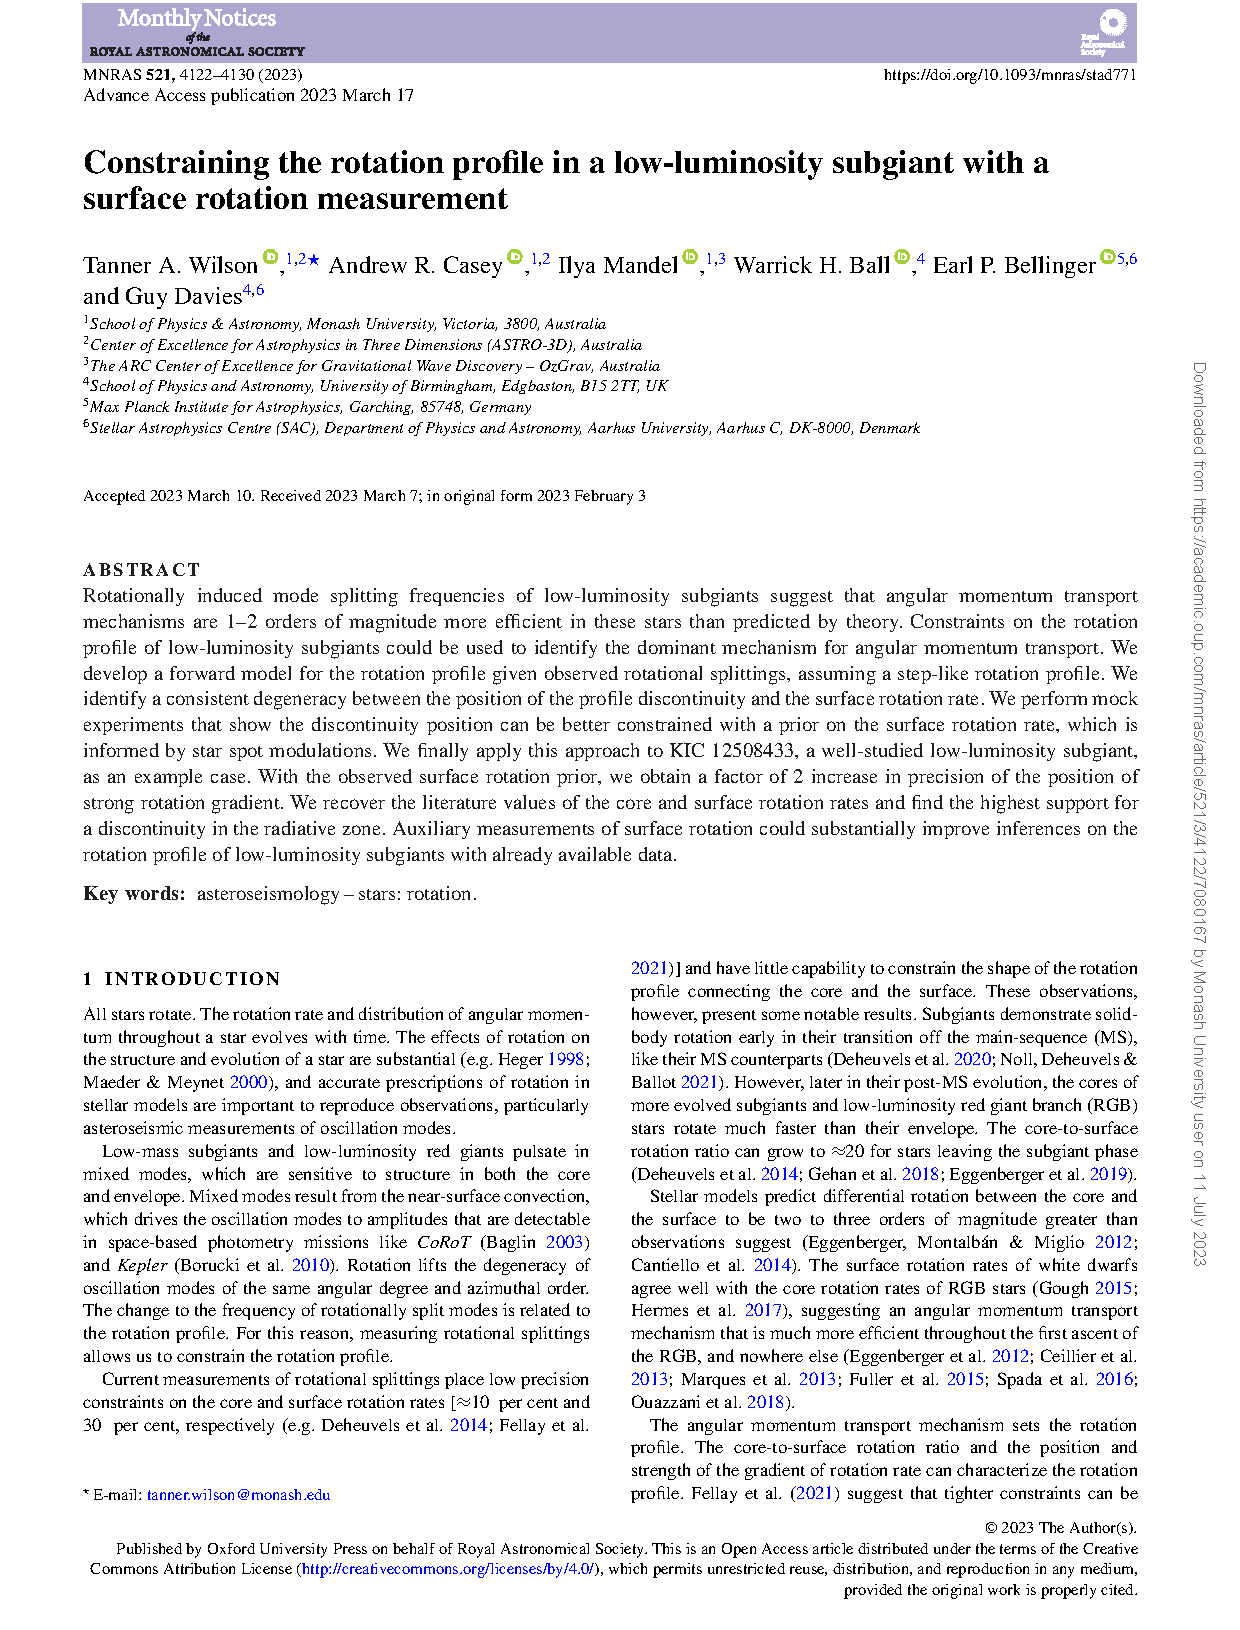
\includepdf[pages =6, addtolist = {6,figure, Posterior distributions of core rotation rate $\Omega_c${,} the surface rotation rate $\Omega_s${,} and the discontinuity position $p$ given the observed $l=\{1{,}2\}$ rotational splittings of KIC 12508433 and assuming a rotation profile with a step function. , f1, 6,figure, Posteriors on step profile parameters given the rotational splittings of KIC 12508433 and informed prior on surface rotation rate from \citep{garcia_rotation_2014}. ,f1, 6, table, Best-fitting rotation profile parameters given observed $\ell = 1$ and $2$ rotational splittings of KIC~12508433 from optimally localised averages (OLA) \citep{deheuvels_seismic_2014} and forward modelling with flat and informed ($\Omega_s/2\pi = 172 \pm 21$ nHz) priors., t1},addtotoc = {6,section,1,Conclusions,p1}, scale=0.9,offset=65 -50,fitpaper=true]{Chapters/stad771-TW-subgiant.pdf}


\includepdf[pages =7, scale=0.9,offset=65 -50]{Chapters/stad771-TW-subgiant.pdf}
\includepdf[pages =8, scale=0.9,offset=65 -50]{Chapters/stad771-TW-subgiant.pdf}
\includepdf[pages =9, scale=0.9,offset=65 -50]{Chapters/stad771-TW-subgiant.pdf}













